\section{Estado del arte}


Como ya se mencionó en la introducción, los datos ómicos abarcan diferentes conjuntos de datos que miden aspectos biológicos desde el ADN, el ARN, proteínas y metabolitos, en los últimos años se han desarrollado herramientas como la creación de bases de datos públicas para facilitar a los investigadores el acceso al análisis de estos datos y el desarrollo de métodos enfocados en la identificación, integración de datos y predicción.

El aprendizaje profundo ha revolucionado el análisis de datos ómicos, obteniendo información compleja y más precisa de conjuntos masivos de datos. Algunas de las principales aplicaciones en la biomedicina son el descubrimiento de biomarcadores, predicción de fenotipos, integración de datos ómicos, diseño de fármacos y regulación genética.

Se destacan algunas estructuras de ANN frecuentemente usadas en el análisis de datos ómicos como las redes neuronales convolucionales en la identificación de patrones espaciales, las redes neuronales recurrentes para modelar secuencias temporales, auto codificadores, redes neuronales profundas, redes generativas y codificadores automáticos variacionales.

Los principales desafíos que se presentan son que se requieren grandes conjuntos de datos para entrenamiento y su procesamiento es una tarea que compromete la eficiencia de la red, sesgo de los datos y la codificación de los datos.

En las siguientes secciones se abordará con más detalle sobre el estado del arte de los datos ómicos, aprendizaje profundo y sus aplicaciones en el análisis de datos ómicos.

\subsection{Datos ómicos}

Las ciencias ómicas se refieren a la evaluación integral o global de una colección de características de un ser vivo, el estudio de genes y proteínas han identificado con éxito, características clave que influyen en la salud y la enfermedad. Los datos ómicos han sido impulsados, debido al desarrollo y disponibilidad de tecnologías de matrices, espectrometría de masas de alto rendimiento y plataformas de secuenciación \citep{hasin2017multi}.

Los sistemas biológicos dependen de la transferencia de información de los ácidos nucleicos a las proteínas y metabolitos para dar forma a la función y fenotipo, es por esto que el estudio de las enfermedades es el resultado de procesos complejos y heterogéneos \citep{kim2018data}. Los datos ómicos son utilizados para el análisis de valores atípicos en una secuencia, lo cual puede indicar la progresión de una enfermedad y permite aprovecharse como indicadores para un diagnóstico temprano, con esto se pueden perfeccionar los enfoques de detección y diagnóstico, así como también identificar y personalizar intervenciones o tratamientos \citep{krassowski2020state}.

Dentro de las ciencias ómicas frecuentemente utilizadas se encuentran: la genómica, transcriptómica, proteómica y la epigenómica, a continuación se detalla un poco más sobre estas ciencias:

La genómica se encarga de la caracterización del contenido genético de un organismo, típicamente consiste en ADN (ARN en algunos virus), la secuenciación del genoma es utilizada para identificación de nuevos genes y variantes genéticas y mediante estudios de asociación de todo el genoma se relacionan variantes genómicas con estados patológicos u otros fenotipos.

La transcriptómica se centra en el estudio del ARN codificante de proteínas (ARN mensajero), las señales transcriptómicas proporcionan información sobre los genes y mecanismos potenciales implicados en un proceso biológico de interés.

La proteómica estudia las proteínas expresadas, las moléculas fundamentales para la vida y su funcionamiento en los organismos vivos. Esta información tiene el potencial para mejorar la compresión de la biología, el diagnóstico de enfermedades y desarrollo de tratamientos.

La epigenómica aborda la caracterización de todo el genoma, de modificaciones químicas reversibles del ADN o de proteínas asociadas al ADN que afectan la expresión y regulación de genes. Las modificaciones epigenómicas pueden proporcionar información sobre el estado de la enfermedad y/o la exposición ambiental y actuar como rasgos hereditarios.

Uno de los aspectos actuales más destacados en la investigación ómica es la integración de datos ómicos (multiómica) de diferentes niveles moleculares con el fin de obtener una visión holística de los sistemas biológicos. Se han encontrado desafíos en la integración de datos como la heterogeneidad de datos, la fata de estándares de datos y la complejidad computacional.

\subsubsection{Análisis de datos ómicos}

La tecnología de análisis de datos ómicos ha cambiado la forma en la que se estudian las enfermedades, permitiendo conocer los cambios a nivel molecular que intervienen en diversos padecimientos. A través de los datos ómicos se obtiene una compresión de las causas y mecanismos de las enfermedades, con lo cual se abren oportunidades en aplicaciones de diagnóstico, tratamiento y prevención por medio del descubrimiento de nuevos biomarcadores biológicos \citep{reel2021using}.

Un biomarcador es una sustancia, estructura o proceso que se puede medir en el cuerpo humano o sus productos y puede proporcionar información importante sobre la presencia de una enfermedad o afección \citep{strimbu2010biomarkers}. Los biomarcadores moleculares se descubren analizando grandes cantidades de información proporcionada de diferentes ómicas y estos desempeñan un papel importante en la planificación de medidas y decisiones preventivas para los pacientes en el diagnóstico, pronóstico o predicción. Los biomarcadores de diagnóstico se utilizan para determinar la presencia de una enfermedad en un paciente, por otro lado, los biomarcadores de pronóstico brindan información sobre el resultado general con o sin tratamiento. Los biomarcadores predictivos se utilizan para identificar el riesgo de sufrir algún resultado \citep{carlomagno2017diagnostic}.

Dentro de las principales enfermedades analizadas en omica e identificación de biomarcadores se encuentran:

El cáncer debido a que es una de las principales causas de muerte en el mundo y la ómica ha contribuido significativamente a la compresión de su complejidad \citep{sarmiento2020aplicaciones}. En el diagnóstico, el análisis ómico ha permitido la identificación de biomarcadores moleculares para la detección de cáncer en una etapa temprana, incluso antes de la presencia de síntomas. En el pronóstico se puede predecir el curso de la enfermedad y la probabilidad de respuesta al tratamiento, la expresión genética de ciertos genes puede usarse para predecir el riesgo de recurrencia del cáncer. En el tratamiento se han impulsado el desarrollo de terapias dirigidas, que se enfocan en las mutaciones genéticas especificas que impulsan el crecimiento del cáncer. Y en la prevención se usa para la identificación de individuos con un alto riesgo de desarrollar cáncer, lo que permite implementar estrategias de prevención personalizada \citep{munir2019cancer}.

Las enfermedades cardiovasculares, como los ataques cardiacos y los accidentes cerebrovasculares, son otra de las causas de muerte a nivel global. En el diagnóstico se puede predecir el riesgo de presentar enfermedades cardiovasculares en el que se analizan los niveles de lipoproteina de baja densidad y de alta densidad que se asocian a un mayor riesgo de enfermedad cardiaca. En el tratamiento, la ómica ha contribuido en el desarrollo de fármacos para implementación en pacientes con dicha patología \citep{pasha2020cardiovascular}. En la prevención se utiliza para identificar en una persona propensa a desarrollar enfermedades cardiovasculares, lo cual permite implementar estrategias de prevención personalizada, como cambios en estilo de vida, dieta saludable y actividad física para reducir el riesgo en individuos con predisposición genética \citep{wang2017detecting}.

Las enfermedades neurodegenerativas, como el Alzheimer y el Parkinson, son un grupo de enfermedades progresivas que afectan el sistema nervioso central y provocan una perdida progresiva de la función cerebral. La ómica en el diagnóstico permite identificar biomarcadores asociados con estas enfermedades, el pronóstico permite conocer la progresión de la enfermedad y predecir la tasa de deterioro cognitivo, en el tratamiento permite el desarrollo de fármacos que permitan tratar estas enfermedades y la prevención para identificar individuos con un alto riesgo de desarrollo de este tipo de enfermedades, lo que permite implementar estrategias de prevención personalizadas \citep{erdacs2021neurodegenerative}.

Enfermedades infecciones, normalmente causadas por patógenos como virus, bacterias y parásitos, que es un problema de salud publica recurrente e importante, la ómica en el diagnóstico permite identificar los biomarcadores por medio de detección genética viral, en el tratamiento de para desarrollo de nuevos antibióticos y antivirales más efectivos y en la prevención para identificar a las personas más propensas a desarrollar enfermedades infecciones e implementar estrategias como las vacunas \citep{chae2018predicting}.



\subsubsection{Bases de datos ómicos}

La producción de datos ómicos incrementa cada año. es por esto que se han establecido diversas bases de datos bioinformáticas que contienen diferentes tipos de datos moleculares, como secuencias de ADN, perfiles de expresión genética, datos de metilación de ADN y variantes genéticas. La adquisición de datos para entrenamiento y validación de los modelos de aprendizaje profundo ya no se considera un problema, en la Tabla \ref{tab:bases_de_datos} siguiente se presentan varias bases de datos de uso común en la rama ómica \citep{zhang2019deep}.

\begin{table}[h!]
    \scriptsize
    \centering
    \caption{Bases de datos ómicos disponibles de libre acceso}
    
    \begin{tabular}{
    >{\centering\arraybackslash}m{6cm} 
    >{\centering\arraybackslash}m{3cm}}
\hline 
        \textbf{Enfoque de la base de datos} & 
        \textbf{Nombre}
\\      
    \hline \hline 

     Datos de genoma &
    {\href{https://www.ncbi.nlm.nih.gov/genome}{NCBI}}
    \\
    &
     {\href{https://www.ensembl.org/index.html}{Ensembl}}
     \\
      &
      {\href{https://www.ensembl.org/index.html}{UCSC}}
     \\
\hline
      Secuenciación de genoma de tipos de cáncer &
     {\href{https://portal.gdc.cancer.gov/}{TCGA}}
    \\
    \\
\hline
      Secuencias de ácidos nucleicos
     &
     {\href{https://www.ebi.ac.uk/ena/browser/home}{ENA}}
     \\
     &
     {\href{https://www.ncbi.nlm.nih.gov/genbank/}{GenBank}} 
     \\
     &
     {\href{https://www.ddbj.nig.ac.jp/index-e.html}{DDBJ}}
     \\
\hline
     Secuencias de proteínas &
     {\href{https://www.uniprot.org/uniprotkb/P51587/entry}{Swiss-prot}}
\\ 
%----------------------------------------------------------
     &
     {\href{https://proteininformationresource.org/}{PIRR}}
     \\
\hline 
     Estructura proteínicas
     &
     {\href{https://www.rcsb.org/pdb}{PDB}}
     \\
\hline     
     Clasificación de estructuras proteínicas &
     {\href{https://scop.berkeley.edu/}{SCOPe}}
     \\
     &
{\href{http://www.cathdb.info/}{CATH}}
     \\
    \hline 
    \end{tabular}
    \label{tab:bases_de_datos}
\end{table}

Este tipo de datos comúnmente tienen formatos del tipo fasta, fastaq, gff2, bed, etc. Propios de su estándar industrial, para aplicación de aprendizaje profundo puede ser necesario conocer lenguajes de programación como Perl, R o Python para la extracción de información y posteriormente ordenar los datos en una forma que los modelos de aprendizaje profundo puedan interpretar como matrices y vectores.

Actualmente, existe una gran cantidad de datos ómicos para diversas aplicaciones en la investigación médica actual impulsadas por tecnología de secuenciación de los cuales destaca la investigación del cáncer que es uno de los mayores proveedores de datos ómicos moleculares a gran escala, que proporciona soporte de datos integral desde la perspectiva de diferentes procesos biológicos y ayuda a explorar la patogénesis de todo tipo de cáncer y tumores cancerígenos \citep{li2024avbae}.

\subsection{Aprendizaje profundo}

El aprendizaje profundo es un campo de la inteligencia artificial, se ha impulsado debido a la disponibilidad de conjuntos de datos, recursos computacionales y algoritmos innovadores. El campo de aplicación es amplio, pero se tienen investigación importante recientes como:

\begin{itemize}

   \addtolength{\itemsep}{-4mm} %con esto se ajusta el interlineado entre la lista
        \item En la ciencia para análisis de conjunto de datos científicos y realizar descubrimientos en las áreas de la física, química y biología.

        \item DL aplicado en atención médica, desarrollando herramientas de diagnóstico y tratamiento para enfermedades como el cáncer, enfermedades cardiacas y enfermedades neurológicas.

    \end{itemize}

\subsubsection{Aprendizaje profundo en ómica}

El DL en el área de la genómica se ha usado para predecir las unidades funcionales de las secuencias de ADN, predecir el dominio de replicación, predicción del factor de transcripción, el punto de iniciación de la transcripción, el promotor, el potenciador y el sitio de borrado del gen \citep{quang2019factornet,umarov2017recognition,zeng2016convolutional,zhang2017titer,min2017predicting,singh2019predicting,lee2015dna}. En los últimos años, se ha impulsado el uso de redes neuronales convolucionales enfocado en la predicción de promotores, potenciadores, dominios de replicación, detección de supresiones genéticas y diferenciación de exones de intrones. El uso de Redes Neuronales Convolucionales (CNN) se ha impulsado en los últimos años en la predicción de promotores, potenciadores, dominio de replicación, detección de supresiones genéticas y diferenciación de exones de intrones.

También se destaca el uso de aprendizaje profundo para predicción de la expresión genética. Esto implica en la predicción del gen objetivo, de la función génica, modelado de redes de regulación génica, etc. En estas aplicaciones, los datos de entrenamiento utilizados frecuentemente son: secuencias de ADN y datos de modificación de histonas. Las redes neuronales especializadas para esta aplicación son las CNN y las RNN \citep{quang2016danq,raza2016recurrent,zhou2015predicting,cuperus2017deep,koh2017denoising}.

Se encuentran trabajos importantes del uso de aprendizaje profundo para explorar genomas y enfermedades epigenéticas y otros campos. Los datos de entrenamiento frecuentemente usados son: el mapa genómico, los perfiles de expresión genética y datos clínicos. En este campo de aplicación los esquemas de redes neuronales es más amplió como CNN, RNN, Auto-codificadores, Redes Generativas \citep{liang2014integrative,yousefi2017predicting,young2017unsupervised}.

El DL en la transcriptómica se analiza la estructura de secuencias de ARN como los sitios de unión de RBP, sitios de empalme alternativo y los tipos de ARN. Para el entrenamiento, los datos frecuentemente utilizados son las secuencias de ARN, estructuras secundarias y terciarias de ARN y CLIP-seq. En estas aplicaciones las redes CNN y RNN son las mas utilizadas \citep{xu2017deep,zhang2017sequence,pan2017rna}.

Las aplicaciones más relevantes es la asociación entre el ARN y las enfermedades o entre el ARN y el diseño de fármacos. Para el entrenamiento de DL se utilizan datos de secuencias de ARN (miRNA-seq), transcriptómica en el mapa genético y datos metilación de ARN. Para estas aplicaciones el uso de esquemas de redes neuronales es más amplio como CNN, RNN, AE y GAN \citep{chaudhary2018deep,yu2018drug,aliper2016deep,bhat2016deepcancer}.

El DL en proteómica se usa en la identificación de estructura de proteínas, como la predicción de la estructura terciaria y secundaria de proteínas, evaluación del modelo de proteínas, predicción del mapa de contacto de proteínas, etc. Los datos que se utilizan en el entrenamiento son la secuencias de aminoácidos, estructuras bidimensionales de proteínas y propiedades fisicoquímicas de aminoácidos. En esta aplicación se encuentran las redes neuronales profundas (DNN) con un cambio al uso de RNN \citep{stahl2017epsilon,li2017deep,spencer2014deep,heffernan2015improving}.

También se destaca el uso de DL en la predicción de la función de proteínas, donde los datos utilizados para el entrenamiento del modelo son secuencias de aminoácidos, la estructura de la proteína e interacciones proteína-proteína, el tipo de redes más usadas son las CNN y las RNN \citep{kulmanov2018deepgo,wang2017musitedeep}.

En la Tabla~\ref{tab:revision} se muestra la revisión de los algoritmos de aprendizaje profundo utilizados para propósitos de clasificación, predicción, codificación de los datos, y el tipo de datos utilizados.

\begin{table}[!h]
    \scriptsize
    \centering
    \caption{Revisión del estado del arte de algoritmos utilizados en clasificación, identificación, codificación y clasificación}
    
    \begin{tabular}{
    >{\centering\arraybackslash}m{2cm} 
    >{\centering\arraybackslash}m{2cm}
    >{\centering\arraybackslash}m{1.2cm} 
    >{\centering\arraybackslash}m{1.25cm}
    >{\centering\arraybackslash}m{1.2cm} 
    >{\centering\arraybackslash}m{2cm}
    >{\centering\arraybackslash}m{1.4cm} 
    >{\centering\arraybackslash}m{1.6cm}
    >{\centering\arraybackslash}m{1.5cm}}
\hline 
        \textbf{\tiny{Algoritmo de DL}} & 
        \textbf{\tiny{Tipo de datos omicos}} &
        \textbf{\tiny{Predicción}}  &
        \textbf{\tiny{Clasificación}}  &
        \textbf{\tiny{Codificación}}  &
        \textbf{\tiny{Preprocesamiento}}  &
        \textbf{\tiny{Entrenamiento y validación}}  &
        \textbf{\tiny{Propósito}}  &
        \textbf{\tiny{Referencia}}
\\      
    \hline \hline 

    \tiny{MLP (perceptron multicapa), CNN} &
    \tiny{Transcriptómico, Metabolómicos} &
    x &
    x &
    x &
    x &
    &
    \tiny{Clasificación de etapas de cáncer} &
    \tiny{\citep{yu2019architectures}}
\\ 
    \tiny{XomiVAE} &
    \tiny{Genomico} &
     &
    x &
    x &
    x &
    x &
    \tiny{Clasificación de tipo de tumores} &
    \tiny{\citep{withnell2021xomivae}}
\\ 
    \tiny{Auto Encoder} &
    \tiny{Genómico, transcriptomico} &
     &
    x &
    x &
    x &
    x &
    \tiny{Clasificación de tipos de cancer} &
    \tiny{\citep{franco2021performance}}
\\ 
    \tiny{Deep Prog (CNN y ML)} &
    \tiny{Genómico, transcriptomico} &
    x &
    x &
    x &
    x &
    x &
    \tiny{Clasificación de tipos de cancer} &
    \tiny{\citep{poirion2021deepprog}}
\\
    \tiny{FactorNet (CNN)} &
    \tiny{Genómico, transcriptomico} &
    x &
     &
     &
    x &
    x &
    \tiny{Predicción de factores de transcripción} &
    \tiny{\citep{quang2019factornet}}
\\
    \tiny{CNN, AE, RNN} &
    \tiny{Genómico, epigenómico} &
    x &
     &
     &
    x &
    x &
    \tiny{Predicción metástasis cáncer} &
    \tiny{\citep{albaradei2021machine}}
\\
    \tiny{DCAP} &
    \tiny{Genómico, epigenomico} &
    x &
     &
    x &
    x &
    x &
    \tiny{Predicción tipos cáncer} &
    \tiny{\citep{chai2021integrating}}
\\
    \tiny{VAE} &
    \tiny{Genómico, transcriptomico} &
     &
    x &
     &
    x &
    x &
    \tiny{Clasificación de tipos de cáncer} &
    \tiny{\citep{leng2022benchmark}}
\\
    \tiny{AE, VAE, GAN} &
    \tiny{Genómico, epigenómico} &
    x &
     &
    x &
    x &
    x &
    \tiny{Imputacion de datos faltantes} &
    \tiny{\citep{huang2023deep}}
\\
    \tiny{CNN} &
    \tiny{Genómico, transcriptómico, proteómico} &
    x &
    x &
    x &
    x &
    x &
    \tiny{Identificacion de cancer y clasificacion} &
    \tiny{\citep{chuang2021convolutional}}
\\
    \tiny{DCNN} &
    \tiny{Genómico, transcriptómico} &
    x &
    x &
     &
    x &
    x &
    \tiny{Identificación de cáncer y clasificación} &
    \tiny{\citep{ma2018omicsmapnet}}
\\
    \tiny{DNN, CNN} &
    \tiny{Genómico, transcriptómico} &
    x &
     &
     &
     &
     &
    \tiny{Predicción de expresión genética} &
    \tiny{\citep{talukder2021interpretation}}
\\
    \tiny{CNN} &
    \tiny{Genómico} &
    x &
     &
    x &
    x &
     &
    \tiny{Prediccion de variantes no codificantes} &
    \tiny{\citep{eraslan2019deep}}
\\
    \tiny{CNN, RNN, AE, GAN} &
    \tiny{Genómico, transcriptómico} &
    x &
    x &
    x &
    x &
     &
    \tiny{Resolución unicelular} &
    \tiny{\citep{erfanian2023deep}}
\\
    \tiny{DeepMO} &
    \tiny{Genómico, transcriptómico} &
     &
    x &
    x &
    x &
    x &
    \tiny{Clasificación de cáncer} &
    \tiny{\citep{li2020deep}}
\\
    \tiny{MOADLN} &
    \tiny{Genómico, transcriptómico} &
    x &
    x &
     &
    x &
     &
    \tiny{Clasificación de subtipos de cáncer} &
    \tiny{\citep{gong2023multi}}
\\
    \tiny{CNN} &
    \tiny{Genómico, transcriptómico, epigenmico} &
    x &
    x &
    x &
    x &
    x &
    \tiny{Clasificación de cáncer} &
    \tiny{\citep{li2022machine}}
\\
    \tiny{DeepProg} &
    \tiny{Genómico, transcriptómico, epigenomico} &
    x &
    x &
    x &
    x &
     &
    \tiny{Diagnóstico de cáncer} &
    \tiny{\citep{mathema2023deep}}
\\
\hline
    \end{tabular}
    \label{tab:revision}
\end{table}

En la revisión anterior se puede observar que las principales aplicaciones de los datos omicos es enfocado en identificación y diagnóstico de cáncer debido es una de las enfermedades más importantes actualmente, por esto mismo se ha desarrollado una mayor cantidad de bases de datos. El tipo de algoritmos de aprendizaje profundo más utilizados son el CNN en aplicaciones de predicción y clasificación, seguido de las RNN.

\begin{table}[!h]
    \scriptsize
    \centering
    \caption{Bases de datos enfocadas en el análisis de datos omicos de tipos de cáncer.}
    
    \begin{tabular}{
    >{\centering\arraybackslash}m{2cm} 
    >{\centering\arraybackslash}m{3cm}
    >{\centering\arraybackslash}m{2cm} 
    >{\centering\arraybackslash}m{2cm}}
\hline 
    \textbf{Nombre de la base de datos} & 
    \textbf{Tipo de datos} &
    \textbf{Acceso a tipos de cáncer}  &
    \textbf{Formatos de descarga}
\\      
\hline \hline 

    TCGA &
    Genómica, transcriptómica, proteómica, metabolómica &
    33 tipos &
    TSV 
\\
    UCSC Xena &
    Genómica, transcriptómica, Epigenomicos, proteómica &
    50 tipos &
    JSON, TSV, HDF5 
\\
    GEO &
    Genómica, transcriptómica, proteómica &
    20 tipos &
    JSON, TSV, CSV
\\  
    ICGC &
    Genómica, transcriptómica, proteómica, metabolómica &
    50 tipos &
    CSV ,TSV 
\\
    CBioPortal &
    Genómica, transcriptómica, proteómica &
    200 tipos &
    JSON, TSV 
\\
    NCI &
    Genómica, transcriptómica, proteómica &
    30 tipos &
    JSON, TSV 
\\
    CBDiscovery &
    Genómica, transcriptómica, proteómica &
    25 tipos &
    JSON, TSV 
\\
\hline
    \end{tabular}
    \label{tab:base_datos_cancer}
\end{table}

\subsubsection{Aprendizaje profundo en oncología}

El análisis de datos ómicos actualmente se centra en el cáncer y, por lo tanto, se ubica un mayor número de bases de datos genómicos, transcriptómicos, proteómicos y metabolómicos. Esto presenta una ventaja debido a que se tiene un mayor número de datos de entrenamiento y validación para los investigadores que se dedican al desarrollo de algoritmos de aprendizaje profundo. En la Tabla~\ref{tab:base_datos_cancer} se muestran las distintas bases de datos de distintos tipos de cáncer, destacando la TCGA debido a cuenta con una biblioteca para la descarga por lotes de datos y que ha sido de mayor uso en los trabajos de investigación \citep{li2022identification}.


De esta revisión se logra precisar sobre el tipo de datos que se seleccionaran para el diseño del algoritmo de red neuronal, debido a que los datos enfocados en el cáncer cuentan con el mayor número de bases de datos del cual adquirir conjuntos de entrenamiento. En la Tabla~\ref{tab:RevisionCancer} se toman trabajos con este enfoque.

El DL en el estudio de cáncer se centra en tres propósitos principales los cuales son el diagnóstico y pronostico, descubrimiento y desarrollo de fármacos, y en la prediccion de la respuesta a tratamientos (Figura \ref{fig:DL_Oncologia}).

\begin{figure}[!h]
    \centering
    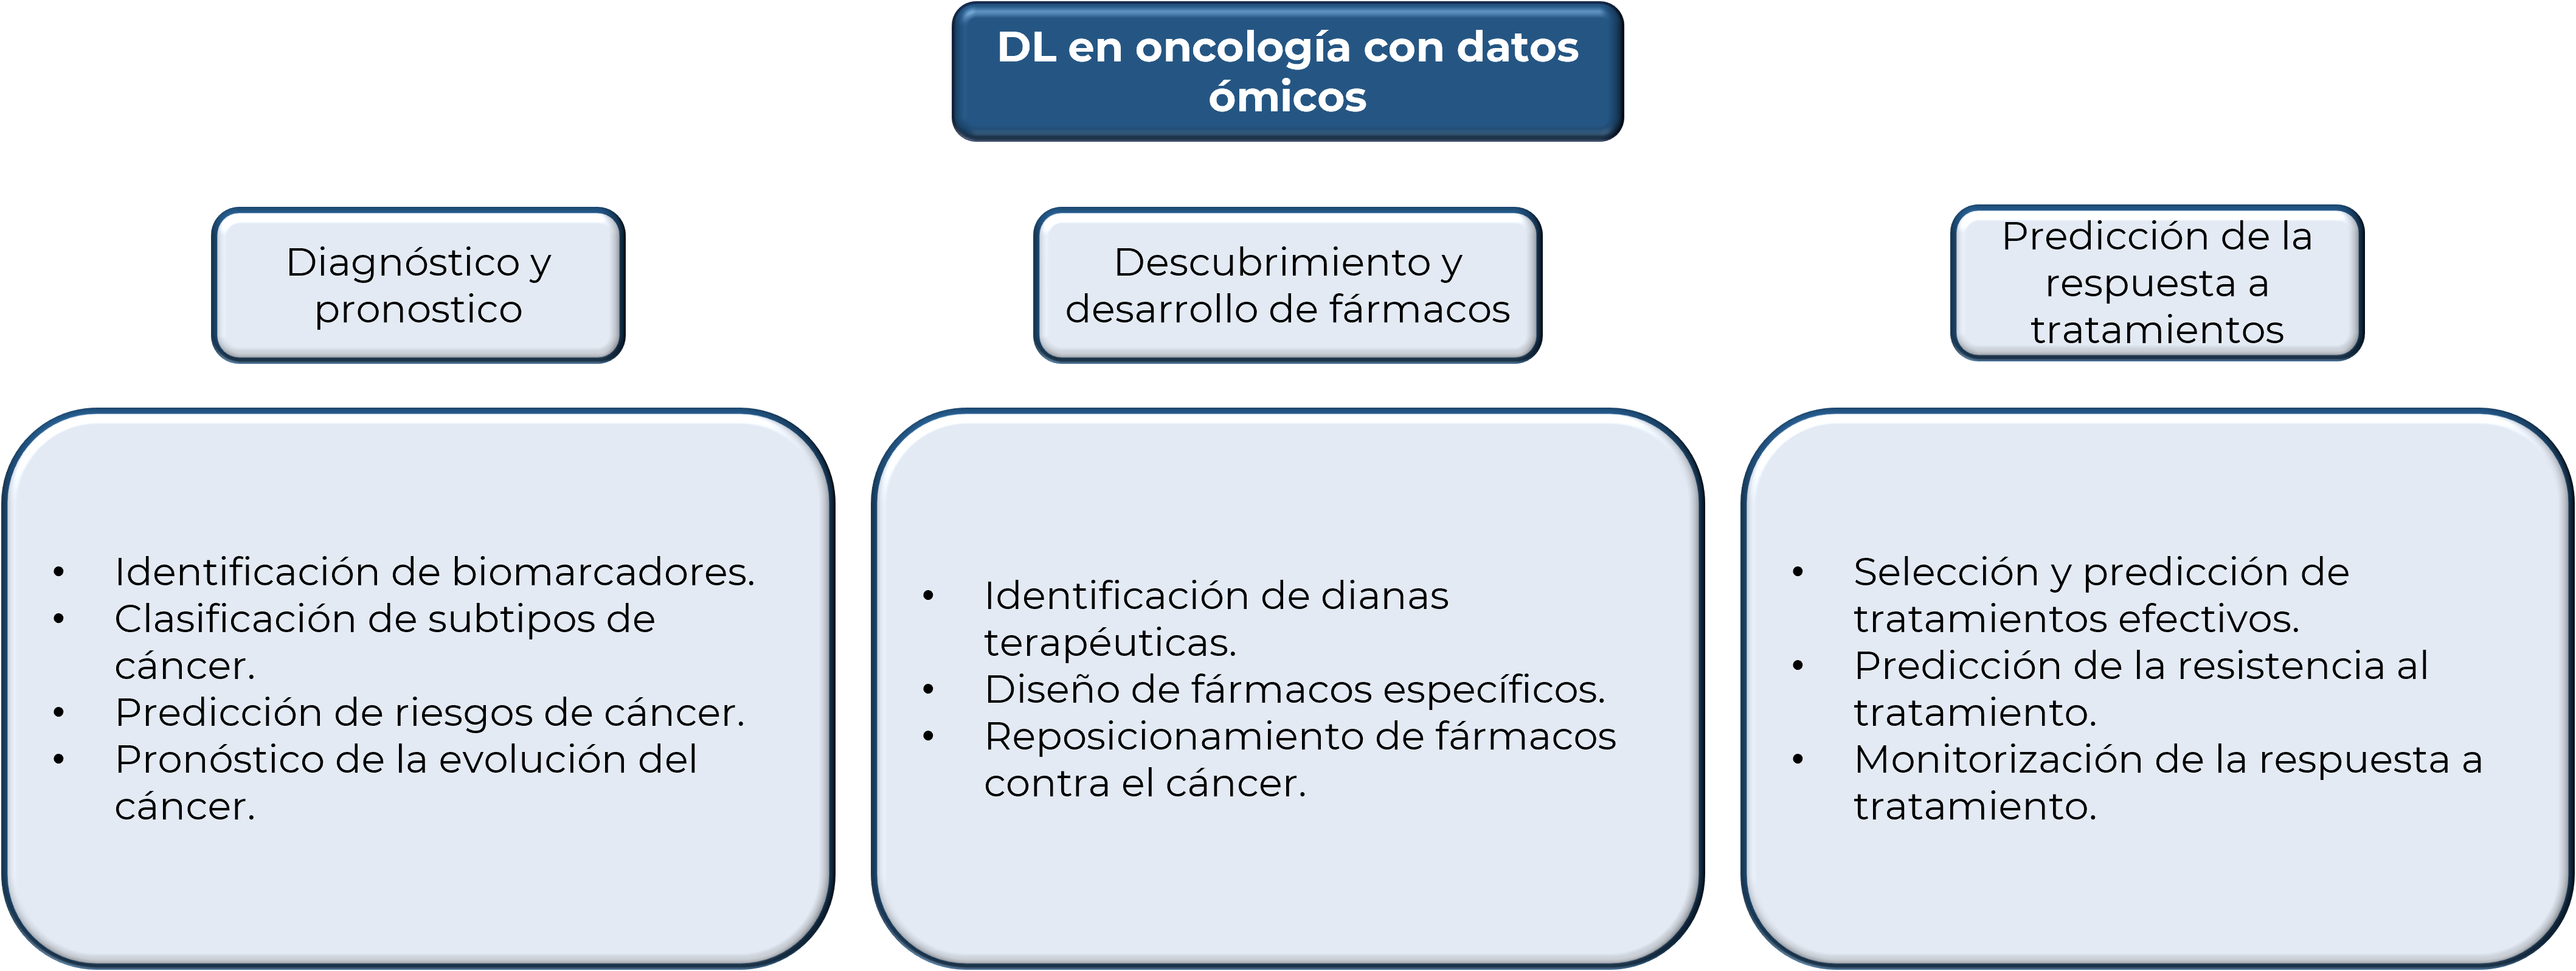
\includegraphics[width=.8\textwidth]{Imagenes/DL_Oncologia.png}
    \caption{Aplicaciones y sus propósitos del aprendizaje profundo en oncología.}
    \label{fig:DL_Oncologia}
\end{figure}

\begin{table}[!h]
    \scriptsize
    \centering
    \caption{Revisión de artículos enfocados en cáncer destacando conjunto de entrenamiento, tipos de datos y base de datos utilizadas.}
    
    \begin{tabular}{
    >{\centering\arraybackslash}m{2cm} 
    >{\centering\arraybackslash}m{2cm}
    >{\centering\arraybackslash}m{2cm} 
    >{\centering\arraybackslash}m{2cm}
    >{\centering\arraybackslash}m{2cm}
    >{\centering\arraybackslash}m{1.5cm} 
    >{\centering\arraybackslash}m{2cm}}
\hline 
    \textbf{Propósito} & 
    \textbf{Conjunto de datos} &
    \textbf{Genómica}  &
    \textbf{Transcriptómica} &
    \textbf{Base de datos} & 
    \textbf{Otros} &
    \textbf{Referencia}
    
\\      
\hline \hline 

    Pronostico de supervivencia &
    15 tipos  &
    x &
    x &
    TCGA &
    &
    \citep{huang2023deep}
\\
\hline
\\
    Clasificación de cáncer &
    11 tipos &
     &
    x &
    TCGA &
    Datos clínicos&
    \citep{chuang2021convolutional}
\\
\hline
\\
    Clasificación de cáncer &
    33 tipos &
    x &
    x &
    TCGA &
    &
    \citep{franco2021performance}
\\
\hline
\\
    Predicción de supervivencia &
    32 conjuntos multiómicos &
    x &
    x &
    TCGA &
    &
    \citep{chuang2021convolutional}
\\
\hline
\\
    Clasificación de cáncer &
    33 tipos &
    x &
    x &
    TCGA &
    &
    \citep{withnell2021xomivae}
\\
\hline
\\
    Clasificación de cáncer y agrupamiento de cáncer&
    5 tipos &
    x &
    x &
    TCGA &
    &
    \citep{chuang2021convolutional}
\\
\hline
\\
    Clasificación de cáncer &
    33 tipos &
    x &
    x &
    TCGA &
    &
    \citep{zhang2019deep}
\\
\hline
\\
    Predicción de supervivencia &
    1 tipo &
    x &
    x &
    TCGA &
    &
    \citep{tong2020deep}
\\
\hline
    \end{tabular}
    \label{tab:RevisionCancer}
\end{table}

El creciente éxito de aprendizaje profundo ha impulsado el desarrollo de software de código abierto, en las que se encuentran las más populares como tensorflow, Caffe, Torch y CNTK. Estas herramientas son compatibles con CPU multinúcleo y GPU multinúcleo \citep{shi2016benchmarking,liu2020application}.

Tensorflow desarrollador por Google integra unidades más comunes en el marco del aprendizaje profundo. Soporta redes actualizadas como CNN y RNN con diferentes configuraciones. Este marco está diseñado para ofrecer flexibilidad, portabilidad y alta eficiencia del hardware equipado.

Caffe desarrollador por Berkeley Vision and Learning Center (BVLC) y es de código abierto desde 2014. Caffe puede procesar 40 millones de imágenes al día con la versión acelerada por GPU en una sola tarjeta GPU NVIDIA k40 o Titan. Con integración cuDNN, se consigue otra aceleración 1.3k \citep{chetlur2014cudnn}.

CNTK es un conjunto de herramientas de redes computacionales unificadas desarrolladas por Microsoft Research, que admite muchas redes neuronales populares. Este marco con múltiples GPU cuenta con un rendimiento bastante aceptable comparándolo con otros \citep{huang2015microsoft}.

Torch es un marco de computación científica que proporciona estructuras de datos para los componentes más útiles en algoritmos de aprendizaje automático, como tensores multidimensionales y operaciones matemáticas sobre ellos.
%-----------------------------------------------


